%%
%% Author: Dario Chinelli
%% begin 2019-12-04
%% last mod 2022-02-02
%%

% Preamble
\documentclass[class=article, crop=false]{standalone}

% Packages
\usepackage[subpreambles=true]{standalone}
\usepackage{import}
\usepackage{graphicx}
\usepackage{amsmath}

% Document
\begin{document}

% Simulations documentation here

\FloatBarrier

\paragraph{Velocities plot}
A significant plot to understand those paths is the one that compares the velocity along the two axes $x$ and $y$.
In this example, it describes how some trajectories are walking left and others are going right, see (Figure \ref{fig:5pids_velhist}).
This plot is made as heat-map, that means each cell gives the intensity of that unique combination of velocities.
\begin{figure}[h]
\centering
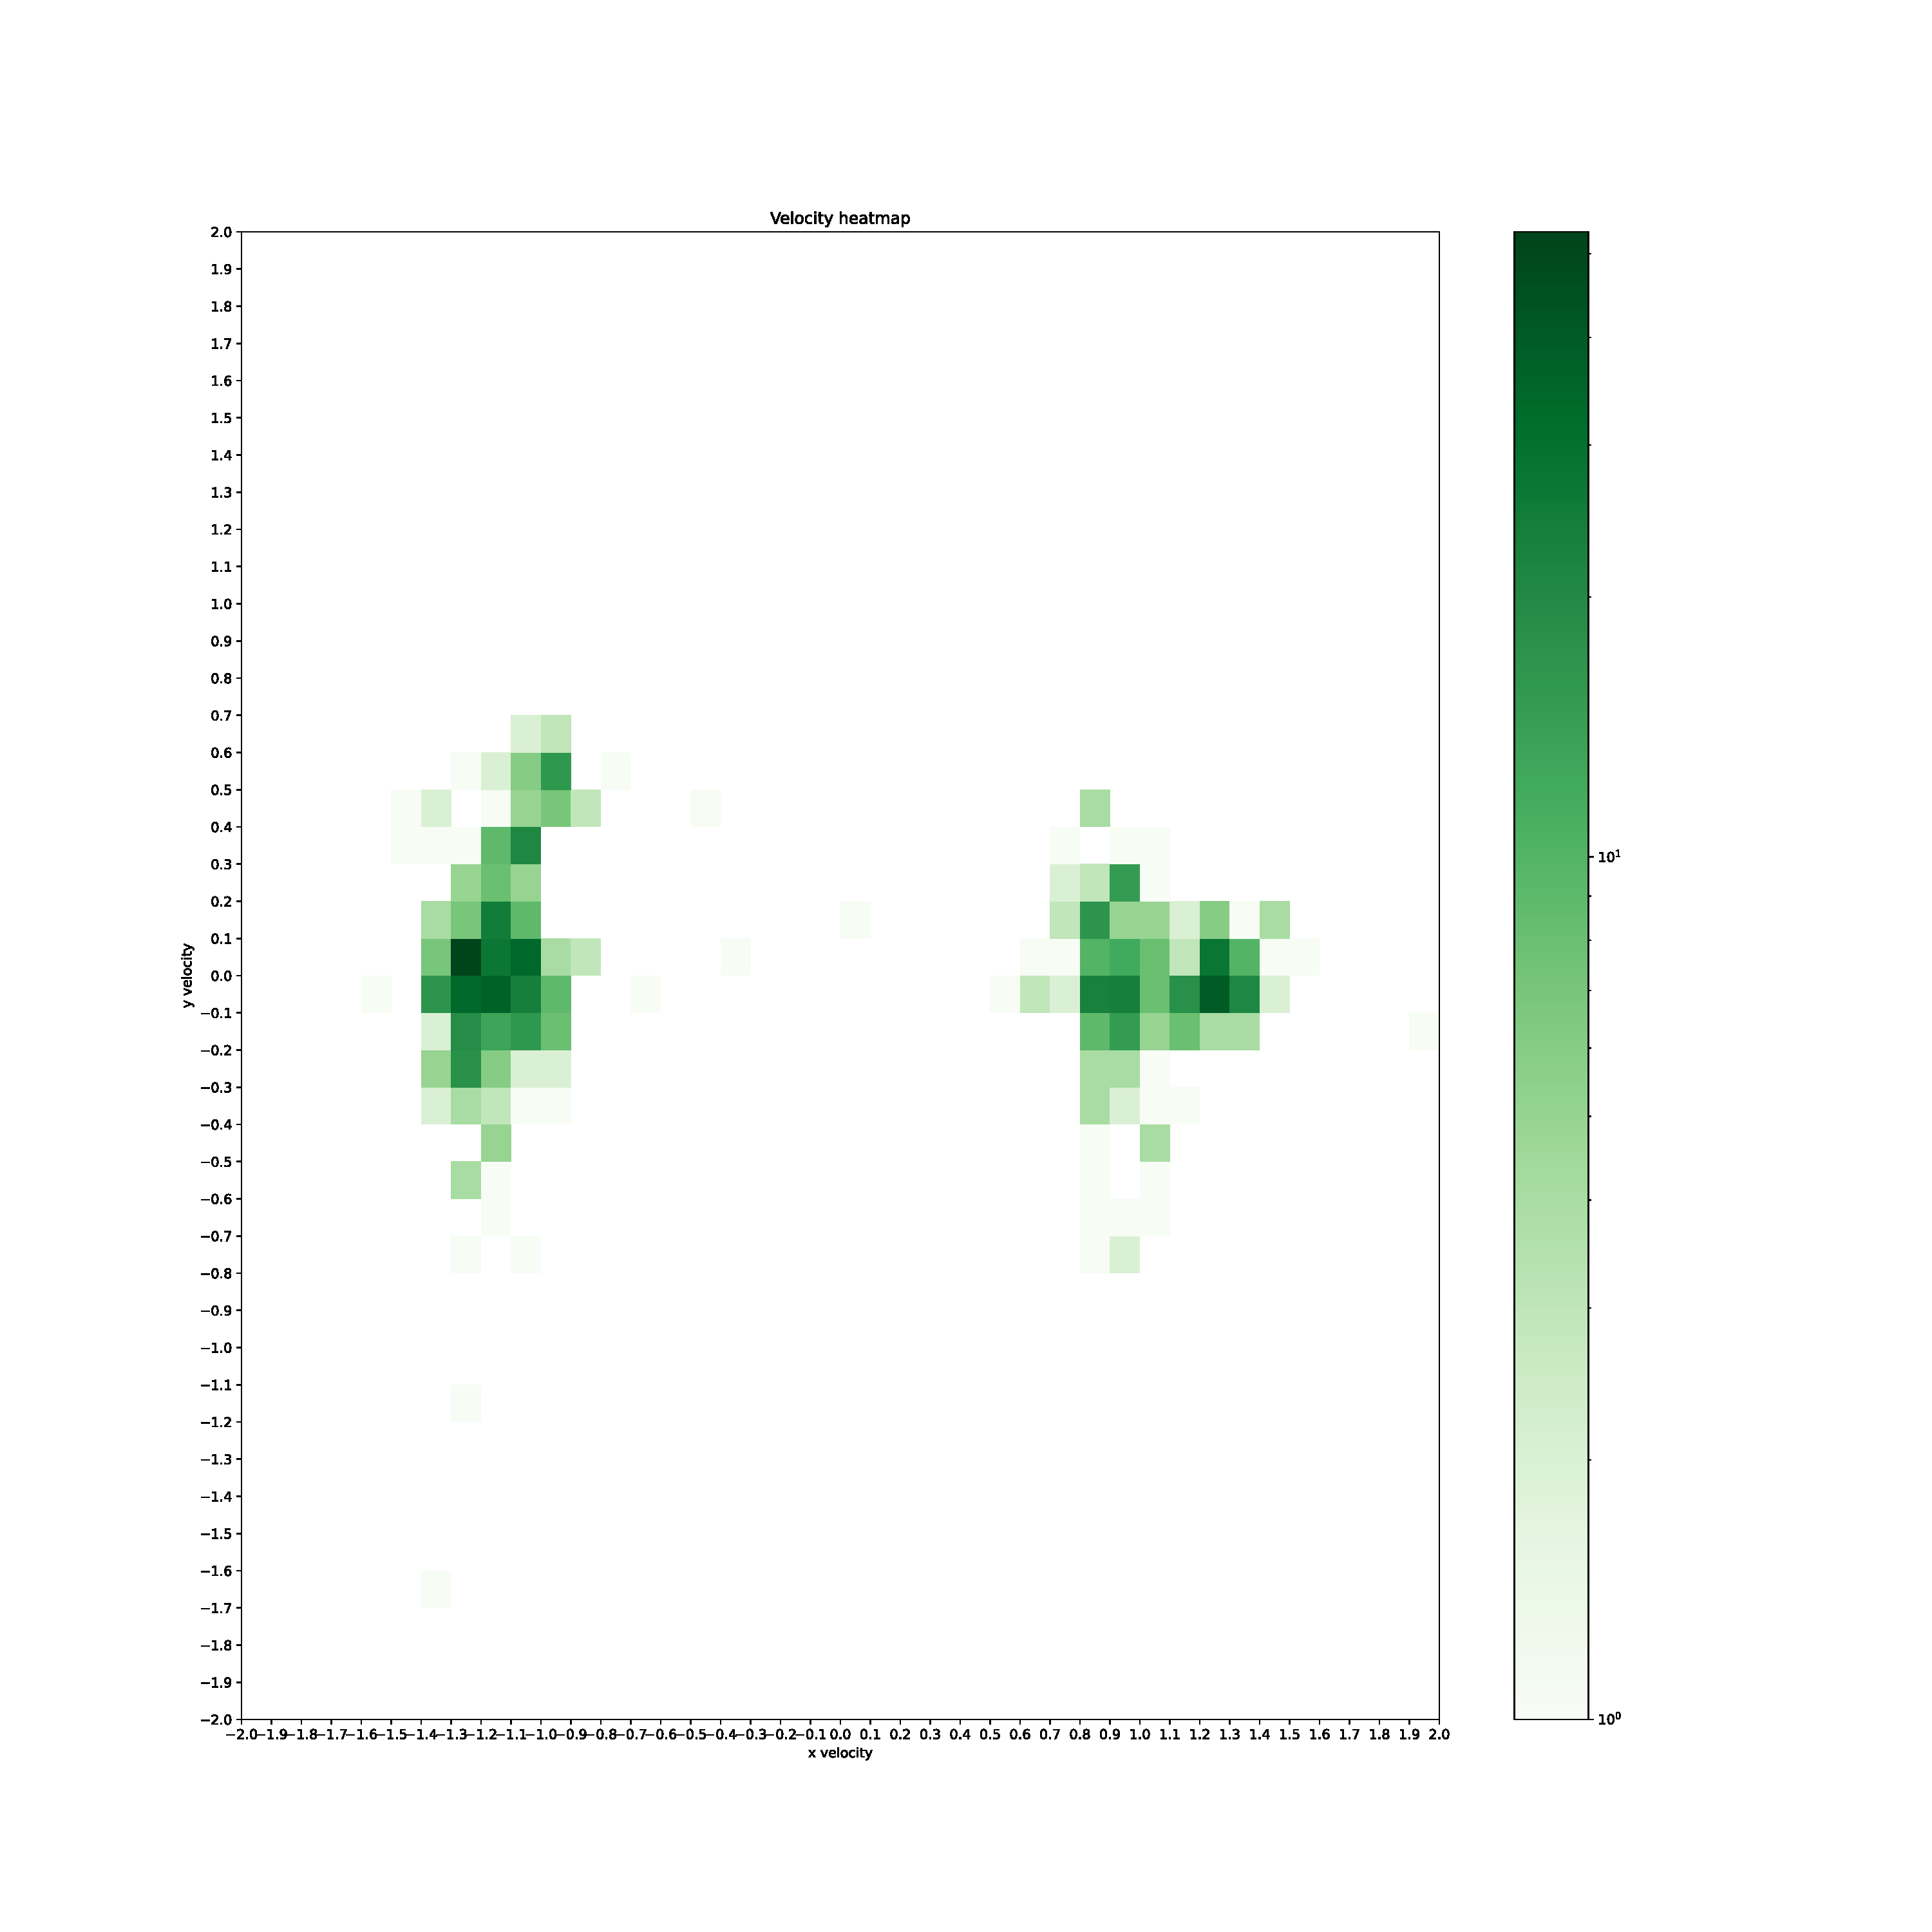
\includegraphics[scale=0.18]{fig/5pids/figure_trainf10_few_trajectories_Dx200_Dy100_VELHIST}
\captionsetup{width=.5\linewidth}
\caption{Comparison between velocity along the two directions $v_x$ and $v_y$.}
\label{fig:5pids_velhist}
\end{figure}
\paragraph{D2Q9 representation}
Another significant plot is the $3\times3$ matrix of figures that follows in (Figure \ref{fig:5pids_D2Q9}), which is composed of nine images.
All those images are referred to the same field, with the same dimensions.
In each of those is plotted the moving probability along just one direction.
The positions of those images are oriented as the $D2Q9$ map, shown in (Figure \ref{fig:D2Q9_k}).
So that the central figure represents the probability to stand still, meanwhile the right-center figure is the probability to move right and so on.
\begin{figure}[h]
\centering
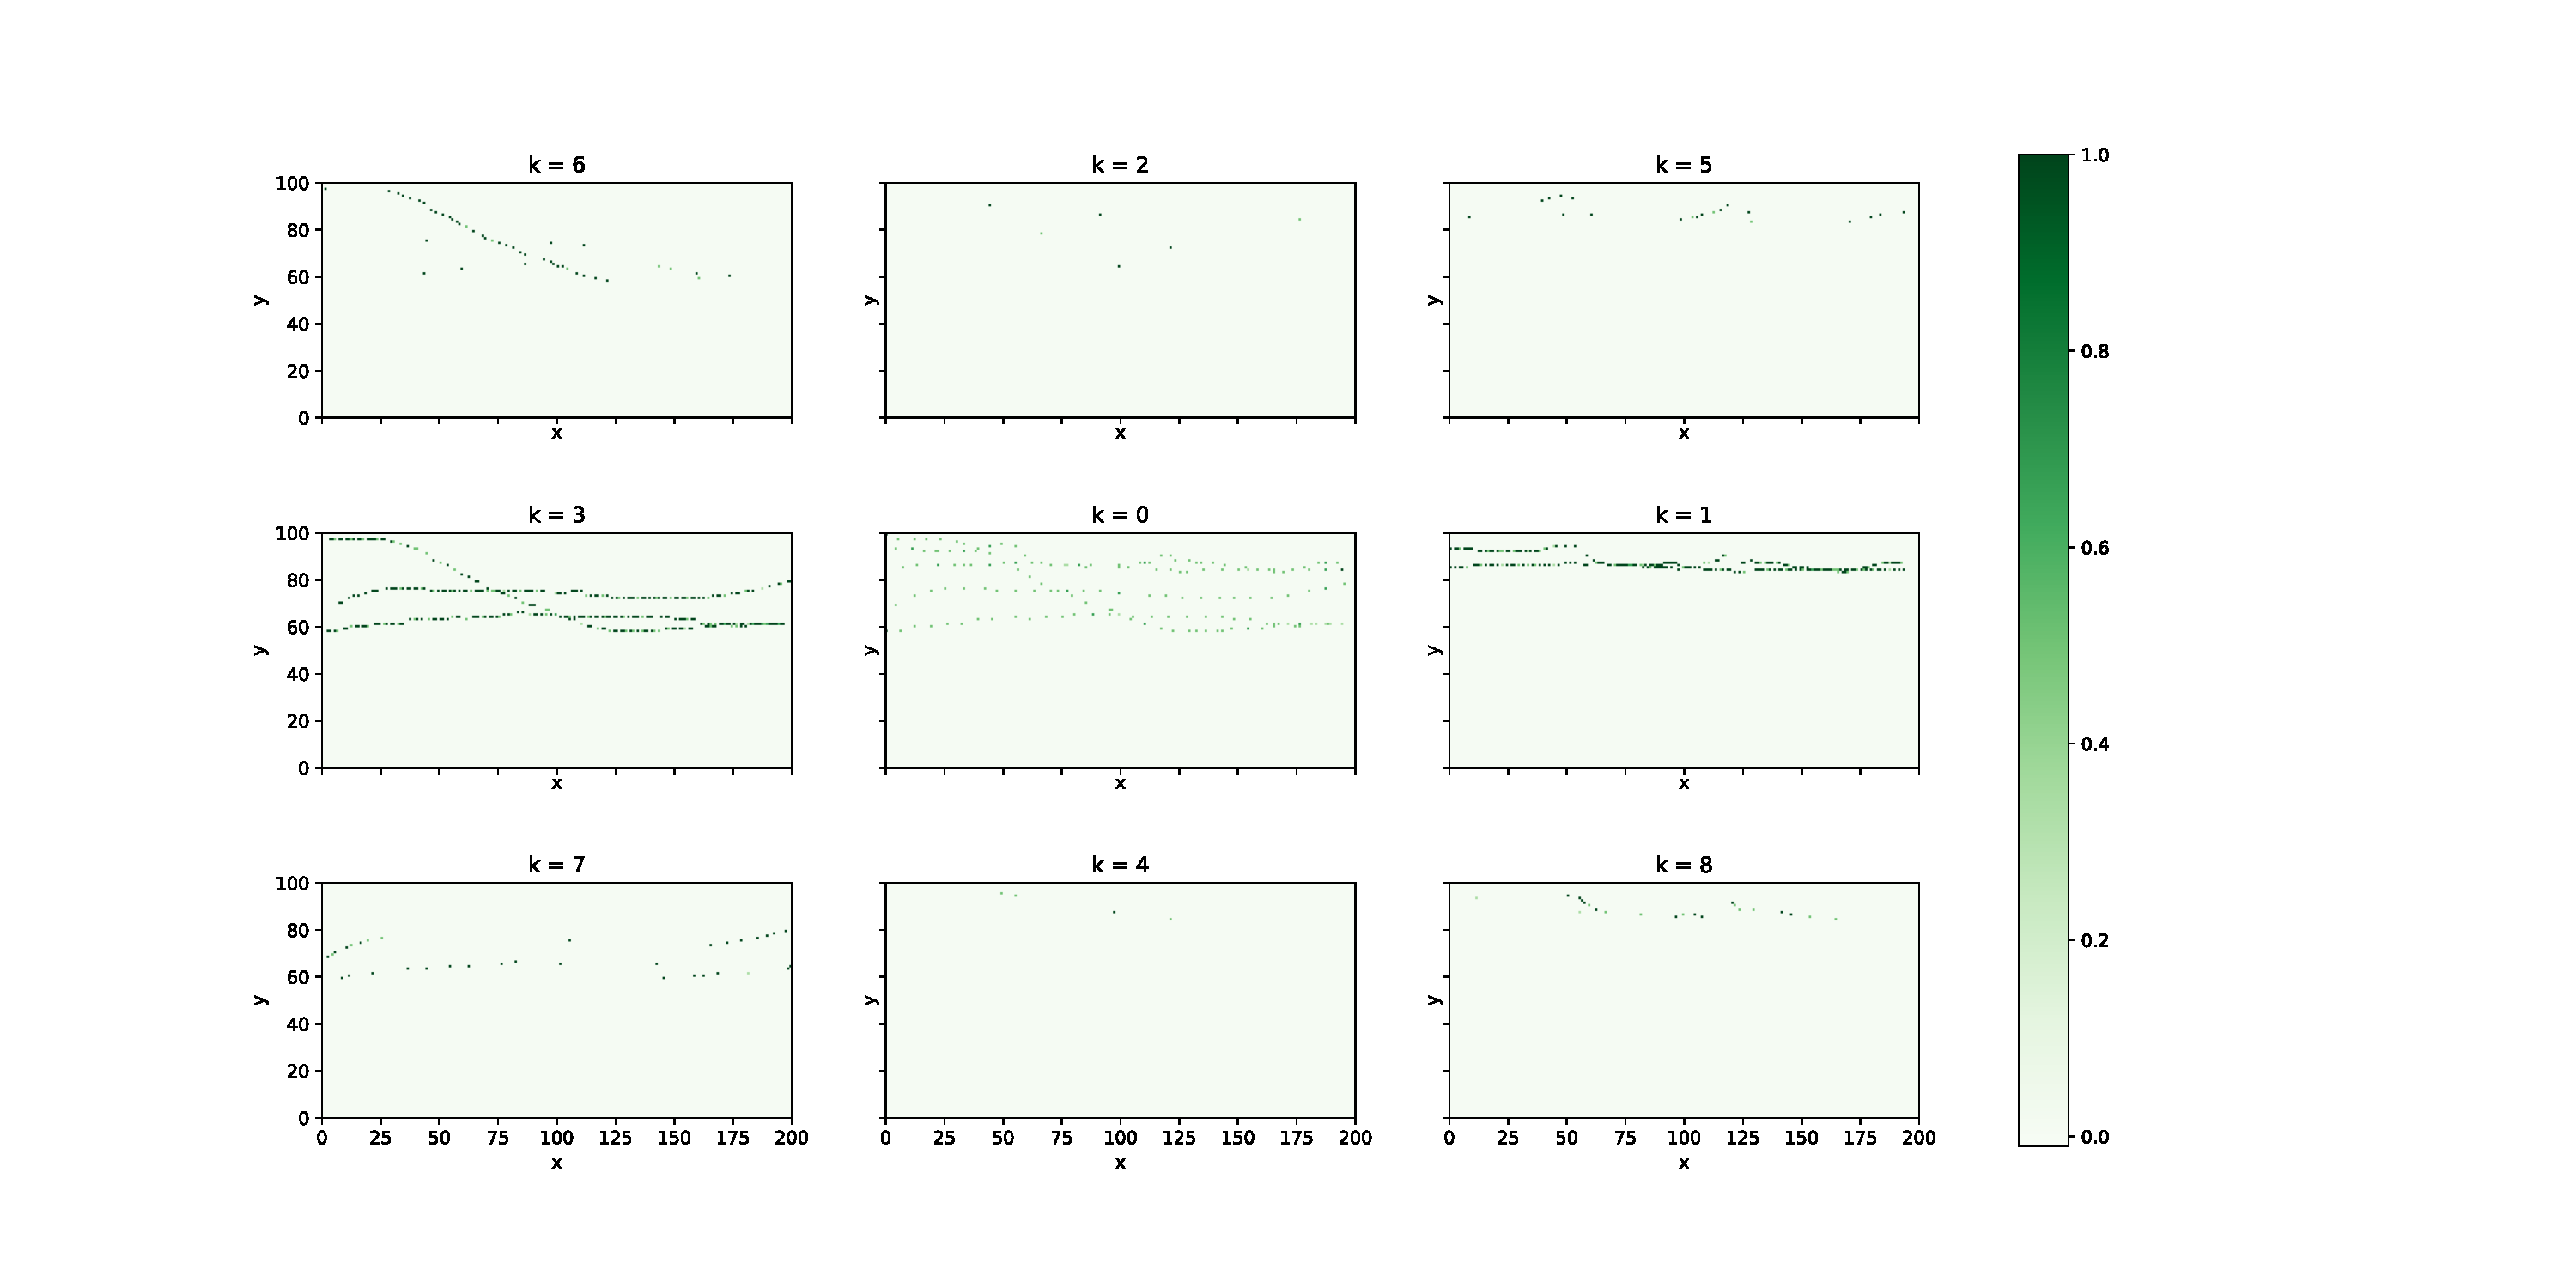
\includegraphics[scale=0.35]{fig/5pids/figure_trainf10_few_trajectories_Dx200_Dy100_D2Q9}
\captionsetup{width=.6\linewidth}
\caption{Representation of the D2Q9 model. Every plot shows the moving probability for each associated direction.}
\label{fig:5pids_D2Q9}
\end{figure}


\FloatBarrier
\subsection{Trajectories simulation}
A good simulation aims to be capable of recreating a realistic path.
In other words, the aim is to make a good prediction on the path chosen by a pedestrian.
To do so, it is necessary to \emph{understand} the trajectories, to \emph{learn} the motion from real-life experiment, before trying to simulate it.

\paragraph{Start positions}
The first step is always the hardest to make, others follow.
The simulation has a start on a cell that is considered part of a group of cells with certain characteristics.
To define this group is necessary to analyze where a real-life trajectory starts.
Let's consider a raw trajectory, a discrete path made from consecutive points.
At every time is associated a position on the $x$-ax and the $y$-ax.
So that a trajectory is described as a group of points in three dimensions, one in time and to in space.
With this definition is easy to define a starting position, asking where is the position when the time is minimum.
The group of the possible \emph{start positions} is created going through all the trajectories and selecting the points that correspond to the minimum time for each of those.

Once the group of start positions is created, it is possible to assign to a synthetic pedestrian its initial position.
In this work, the assignation is made by a random sort from the group named before.
It is possible to select a region of interest in the field.
Combining an arbitrary portion of space and the group of start position and making a new sub-group.
Then the random choice is made from that secondary sub-group.

\paragraph{Step}
The step from the initial position to the second is essentially made with the same procedure as all further steps.
The algorithm takes as input the position, in space and time if necessary.
The tensor $A$ is used to get the probability for each of the nine directions.
So that the initial position, chosen from the group of the start positions, is associated with the time $t=0$.
When this input is given to the algorithm it read the array of the possible transitions from the actual cell to the next.
Then it runs a Monte Carlo through that array and returns the corresponding direction randomly chosen with different probabilities.
For the second position, it will assign time $t=1$ with the new coordinates, running another step.
And so on, one step at the time, moving through the field and increasing the time for each synthetic pedestrian.
It is possible to simulate one trajectory or a hundred, if more than one it will not consider the interactions between those new synthetic.
This fact may be useful to analyze different scenarios in the same crowd.
As also said before, this model takes into account a real-life environment and makes possible the simulations consequentially to the selected scenario.
Choosing a different one led to very different simulations.
Choosing a scenario and running a multitude of simulations lead to a complete \emph{tree} of possible paths.
The path that will be followed more will be the most probable one.

\newpage
\paragraph{Examples to explain the algorithm}
The (Figure \ref{fig:D2Q9_FirstEx}) represents a scenario where, in a certain position, is associated a distribution of probability that make certain the evolution of the system.
In the figure is described that is not possible to move anywhere except to the Right direction.
The second example in (Figure \ref{fig:D2Q9_SecondEx}) is given a different probability distribution.
If in a certain position $(x_0, y_0)$ is associated this type of distribution the randomization will be between going Right or going Down with the same probability.
For the third example in (Figure \ref{fig:D2Q9_thirdEx}) lets assume every entry non-zero.
In this case, some of the future positions will have a low probability to happen and others very high.
So that simulating a great number of trajectories will lead to getting some of them "choosing" also the less probable directions.
For sure the most probable choice is to go Right, the second is to go Down and the third in order of probability is to go Right-Down.
All the other directions follow as less probable, but with a non-zero probability.
	\import{draw/}{D2Q9_example_distribution}

\paragraph{Stop the step}
The simulation of a singular pedestrian has to be stopped by some kind of trigger.
The first trigger is applied when the synthetic pedestrian touches the border of the field.
The other trigger used in this work is made by setting the maximum value for the proper time of each synthetic pedestrian.
Both those triggers must stop the counting of synthetic pedestrian's time and stop calculating the next move for those trajectories.
This may lead to a distribution of the trajectories' length.
That is force cut at the upper limit, imposed by the simulation setup, and depends on when every trajectory touches the border.


\FloatBarrier
\subsection{Distribution of probability}
The analysis on the probability distribution tensor makes it possible to determinate \emph{which trajectory is more likely to be chosen}.
This method proposes an approximation for the continuous general problem.
This method is built on a discrete system of time, space and "directions" of the momentum.
With this approximation it is possible to evaluate the probability for a trajectory, starting from a certain position.
So let's assume the initial position as $(x_0, y_0)$, the trajectory $\gamma$ that starts from that point which path well follows?
If a \emph{tensor} of the probability was created before it is possible to calculate the most probable $\gamma$ starting from that point.
Could be also very interesting to change the question to: "how likely is this $\gamma$ that I'm watching"?
The answer to the last question may be satisfied by multiplying the value of each transition from the starting point to the end.

\paragraph{Simplistic example}
Let's take into account the $D2Q9$-model, so that it's defined by a tensor $A_{x y k}$, in reference to the (Chap. \ref{chap:Model_D2Q9}).
Assume a finite grid of cells, a $6\times3$ matrix, where $x$ is horizontal and $y$ is vertical.
Assume that for each position $(x, y)$ is given a vector of \emph{nine} entries with index $k$.
Assume a finite number of possible move distributions, (Equation \ref{equation:simplistic_example_transitions}).
Let's represent the vector in the form of a matrix, referencing to the (Figure \ref{fig:D2Q9_k}), to help visualization.
And call them: $A, B, C, D$, with the following values:
\begin{equation}
\begin{split}
A=
\left(
\begin{array}{ccc}
 0 &  0 & 0  \\
 0 &  0 & 1  \\
 0 &  0 & 0  
\end{array}
\right)
\end{split}\quad
\begin{split}
B=
\left(
\begin{array}{ccc}
 0 &  0 & 0  \\
 0 &  0 & 0.3  \\
 0 &  0 & 0.7  
\end{array}
\right)
\end{split}\quad
\begin{split}
C=
\left(
\begin{array}{ccc}
 0 &  0 & 0.7  \\
 0 &  0 & 0.3  \\
 0 &  0 & 0  
\end{array}
\right)
\end{split}\quad
\begin{split}
D=
\left(
\begin{array}{ccc}
 0 &  0 & 0  \\
 0 &  1 & 0  \\
 0 &  0 & 0  
\end{array}
\right)
\end{split}
\label{equation:simplistic_example_transitions}
\end{equation}
remembering that the sum of the vector's entries must be $1$.
Vector $A$ force the movement to go Right.
Vector $B$ allows two possible directions but going Right is less probable than going Right-Down.
Similarly to the previous, vector $C$ allows two possible directions but going Right is less probable than going Right-Up.
The last vector $D$ imposes to stand still and for the scope of this example is useful to stop the steps.

The discrete space $\Omega_g$ of this example is formed by 18 cells and it's represented in (Figure \ref{fig:simplistic_example_1}), in which one is set the probability distribution.
Let's assume that the first position of a synthetic pedestrian starts from a cell in the first column from the left.
Let's also assume that the scope of this simulation is two starting from the left side of $\Omega_g$ and arriving on the right side.
Not all trajectories are permitted, instead only a few are possible.
All the possible path are showed in (Figure \ref{fig:simplistic_example_2}) with different colors.
When the first position is the middle-left cell the simulation could only evolve in one path, the one represented in blue in the (Figure \ref{fig:simplistic_example_4}).
Defining the path in the figure as $\gamma_0$ and its probability as $p_{\gamma_0}$.
This path has the probability to happen equal to $p_{\gamma_0} = 1$ and no other paths are allowed from this cell.
Meanwhile, from the upper-left cell and the bottom-left cell, three paths are possible, as shown in (Figure \ref{fig:simplistic_example_5}), but not with the same probability.
Lets set names for all the trajectories from this cell:
\begin{itemize}
\item $\gamma_0$ : blue path
\item $\gamma_1$ : green path
\item $\gamma_2$ : orange path
\item $\gamma_3$ : red path
\end{itemize}
the notation for theirs probability is $p_{\gamma_i}$.
Each probability can be derived from the series of products of the values of the corresponding transition.
So that in the previous case would be:
\begin{equation*}
p_{\gamma_0} = 1 \times 1 \times 1 \times 1 \times 1 = 1 = 100 \% \;
\end{equation*}
and in fact $\gamma_0$ is the only one possible path.
In the second case would be instead:
\begin{equation}
\begin{split}
p_{\gamma_1} & = 1 \times 1 \times 0.3 \times 0.3 \times 1 = 0.09 = 9 \% \\
p_{\gamma_2} & = 1 \times 1 \times 0.3 \times 0.7 \times 1 = 0.21 = 21 \% \\
p_{\gamma_3} & = 1 \times 1 \times 0.7 \times 1 \times 1    = 0.70 = 70 \%
\end{split}
\label{equation:simplistic_example_probabilities}
\end{equation}
The (Equation \ref{equation:simplistic_example_probabilities}) explicitly shows all the possibilities.
With this result, it's clear which one is the most probable path in this space.

\begin{figure}[ht]
\begin{minipage}[c]{0.5\linewidth}
\centering
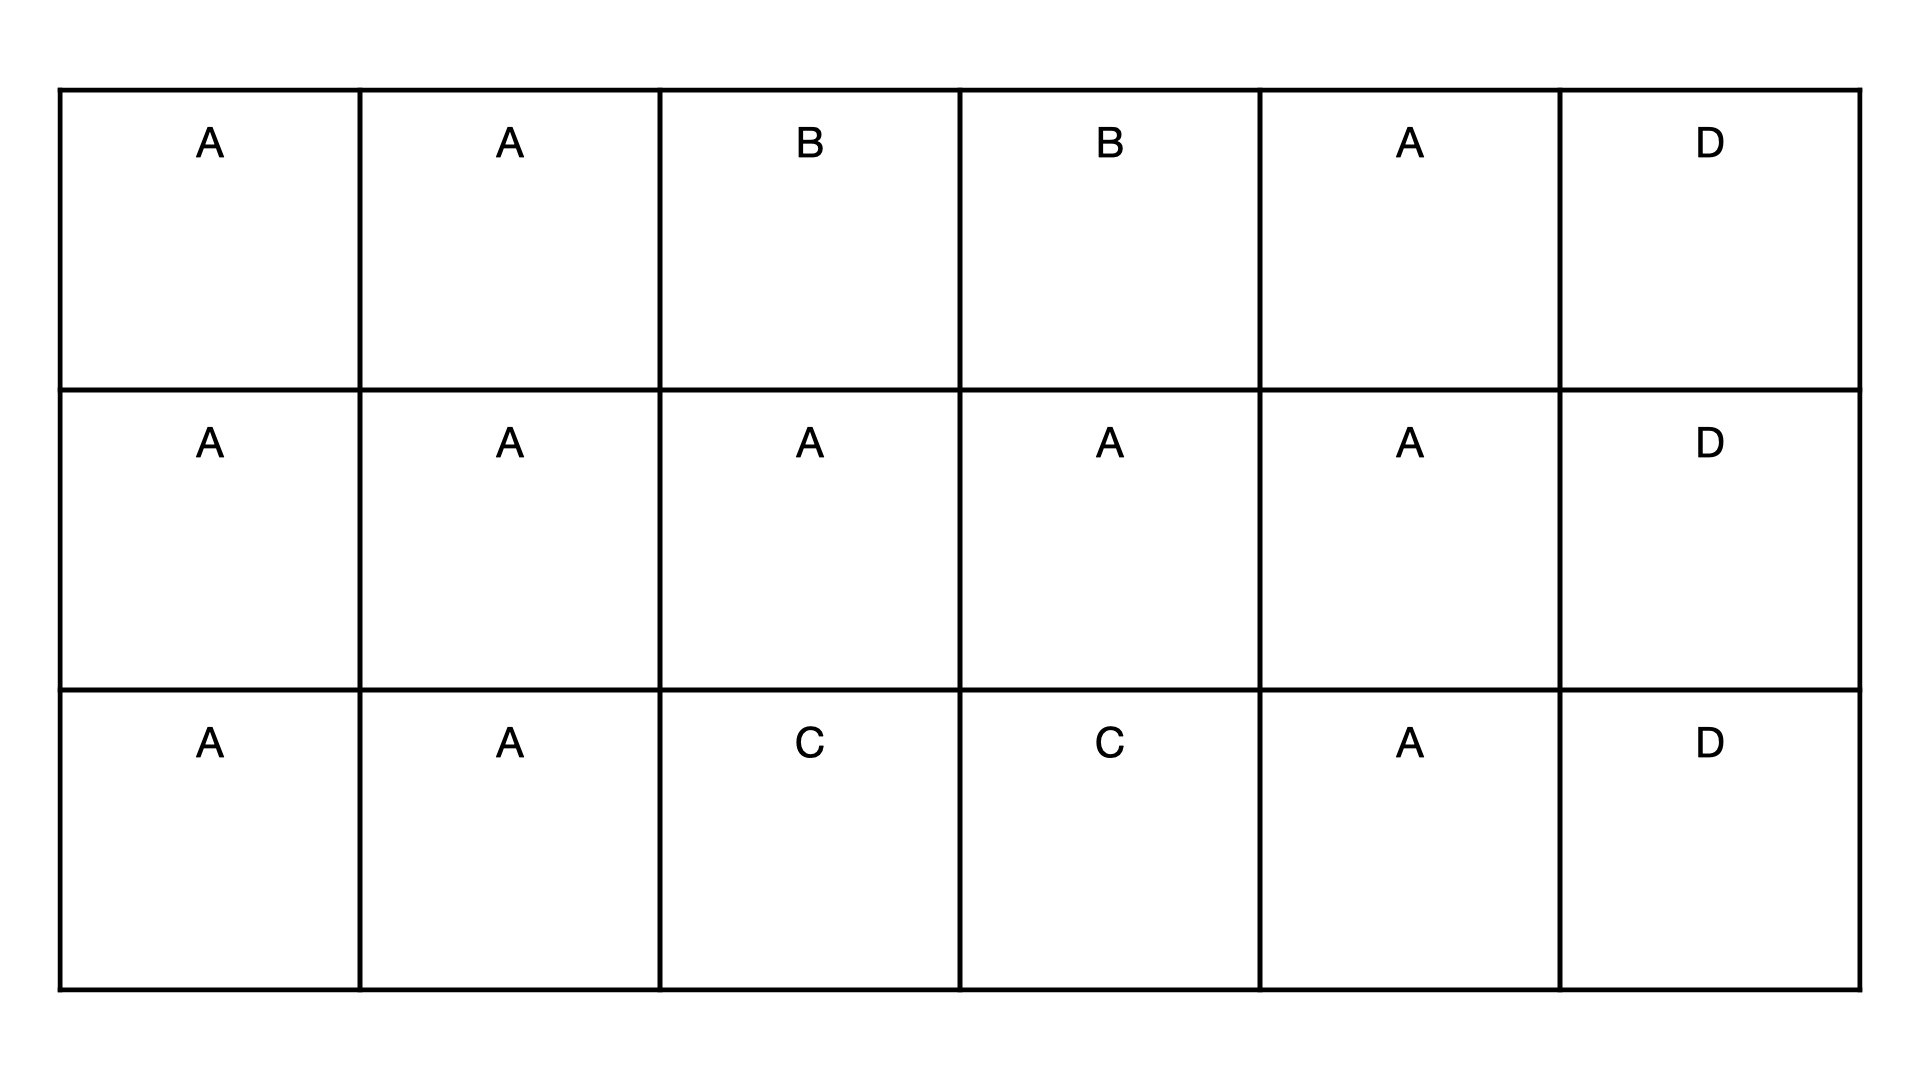
\includegraphics[scale=0.1]{draw/Thesis_plots/Thesis_plots.001}
\captionsetup{width=.8\linewidth}
\caption{Space of the simplistic example. Every letter correspond to a specific distribution of possible transitions, referred to the (Equation \ref{equation:simplistic_example_transitions}).}
\label{fig:simplistic_example_1}
\end{minipage}
\begin{minipage}[c]{0.5\linewidth}
\centering
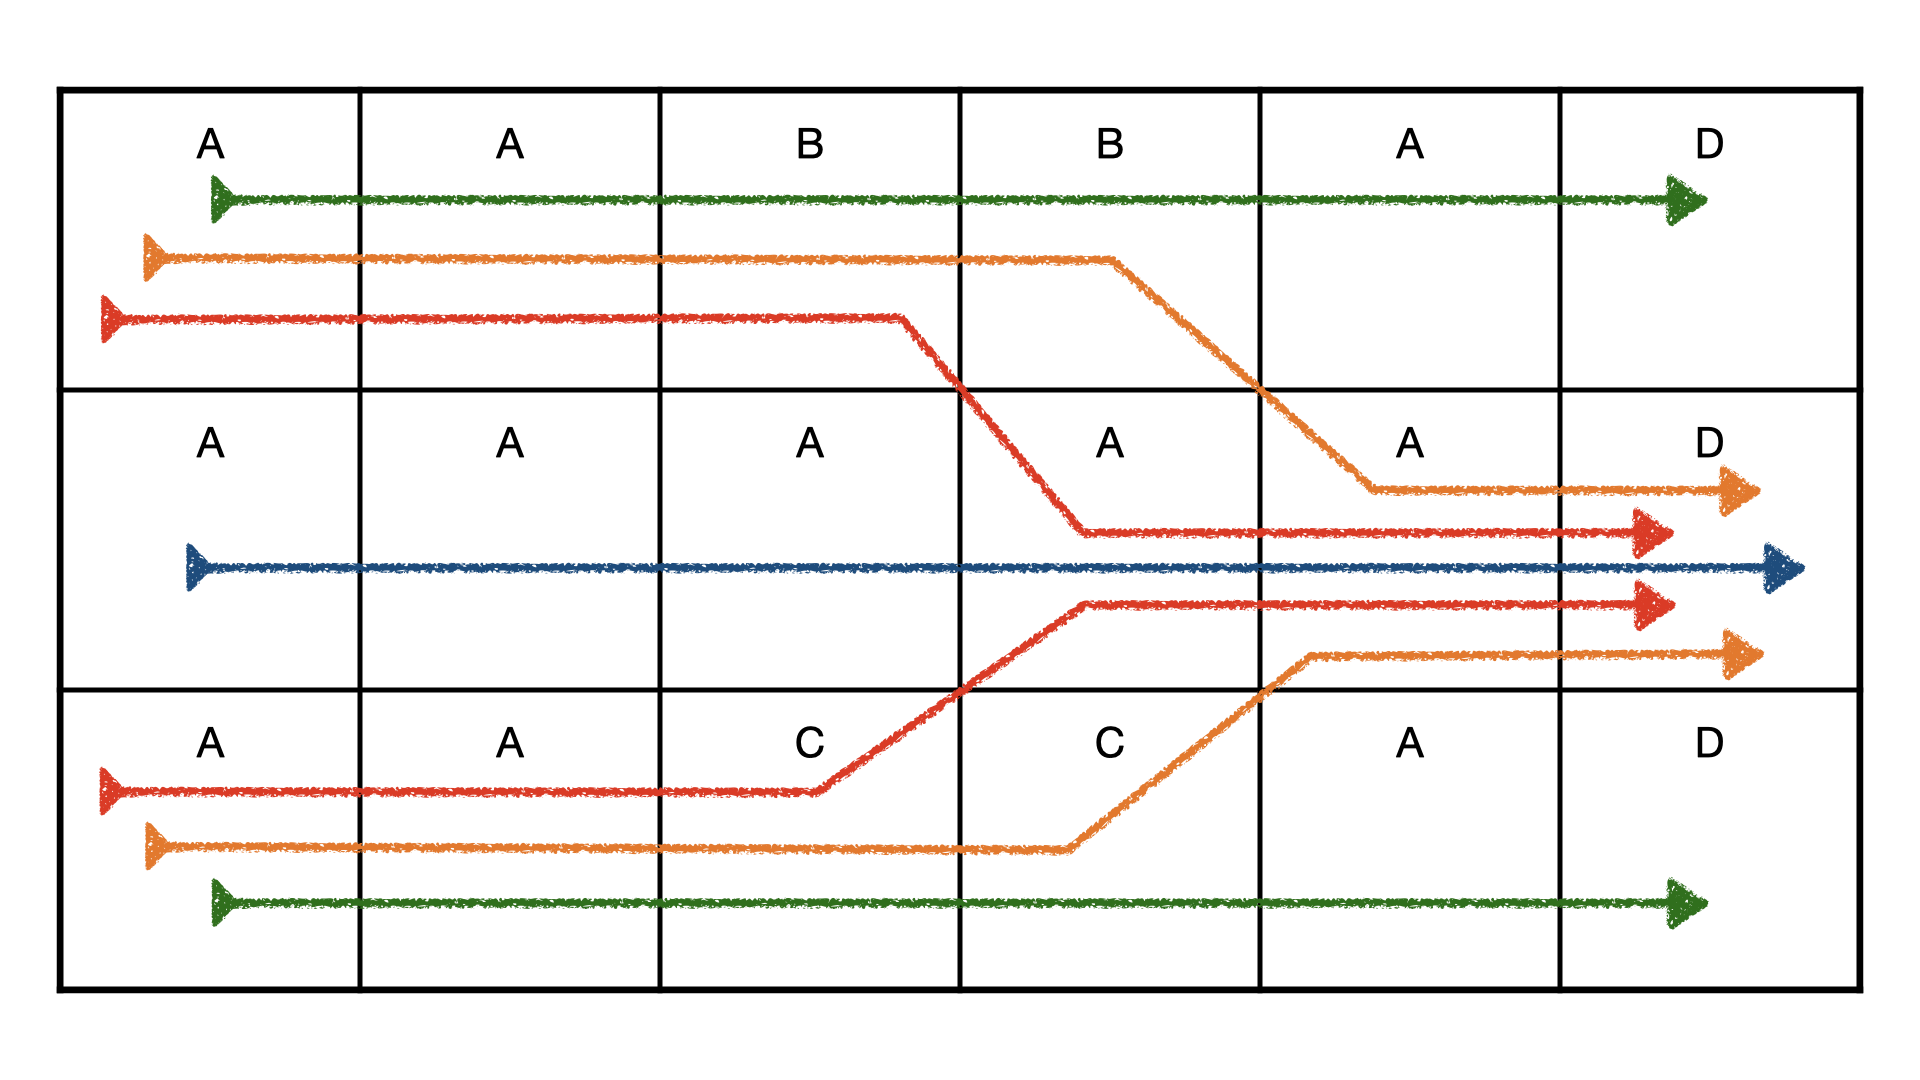
\includegraphics[scale=0.1]{draw/Thesis_plots/Thesis_plots.002}
\captionsetup{width=.8\linewidth}
\caption{All the possible paths that are permitted to travel from the left to the right side of the map $\Omega_g$. Different colors represents different probabilities.}
\label{fig:simplistic_example_2}
\end{minipage}
\begin{minipage}[c]{0.5\linewidth}
\centering
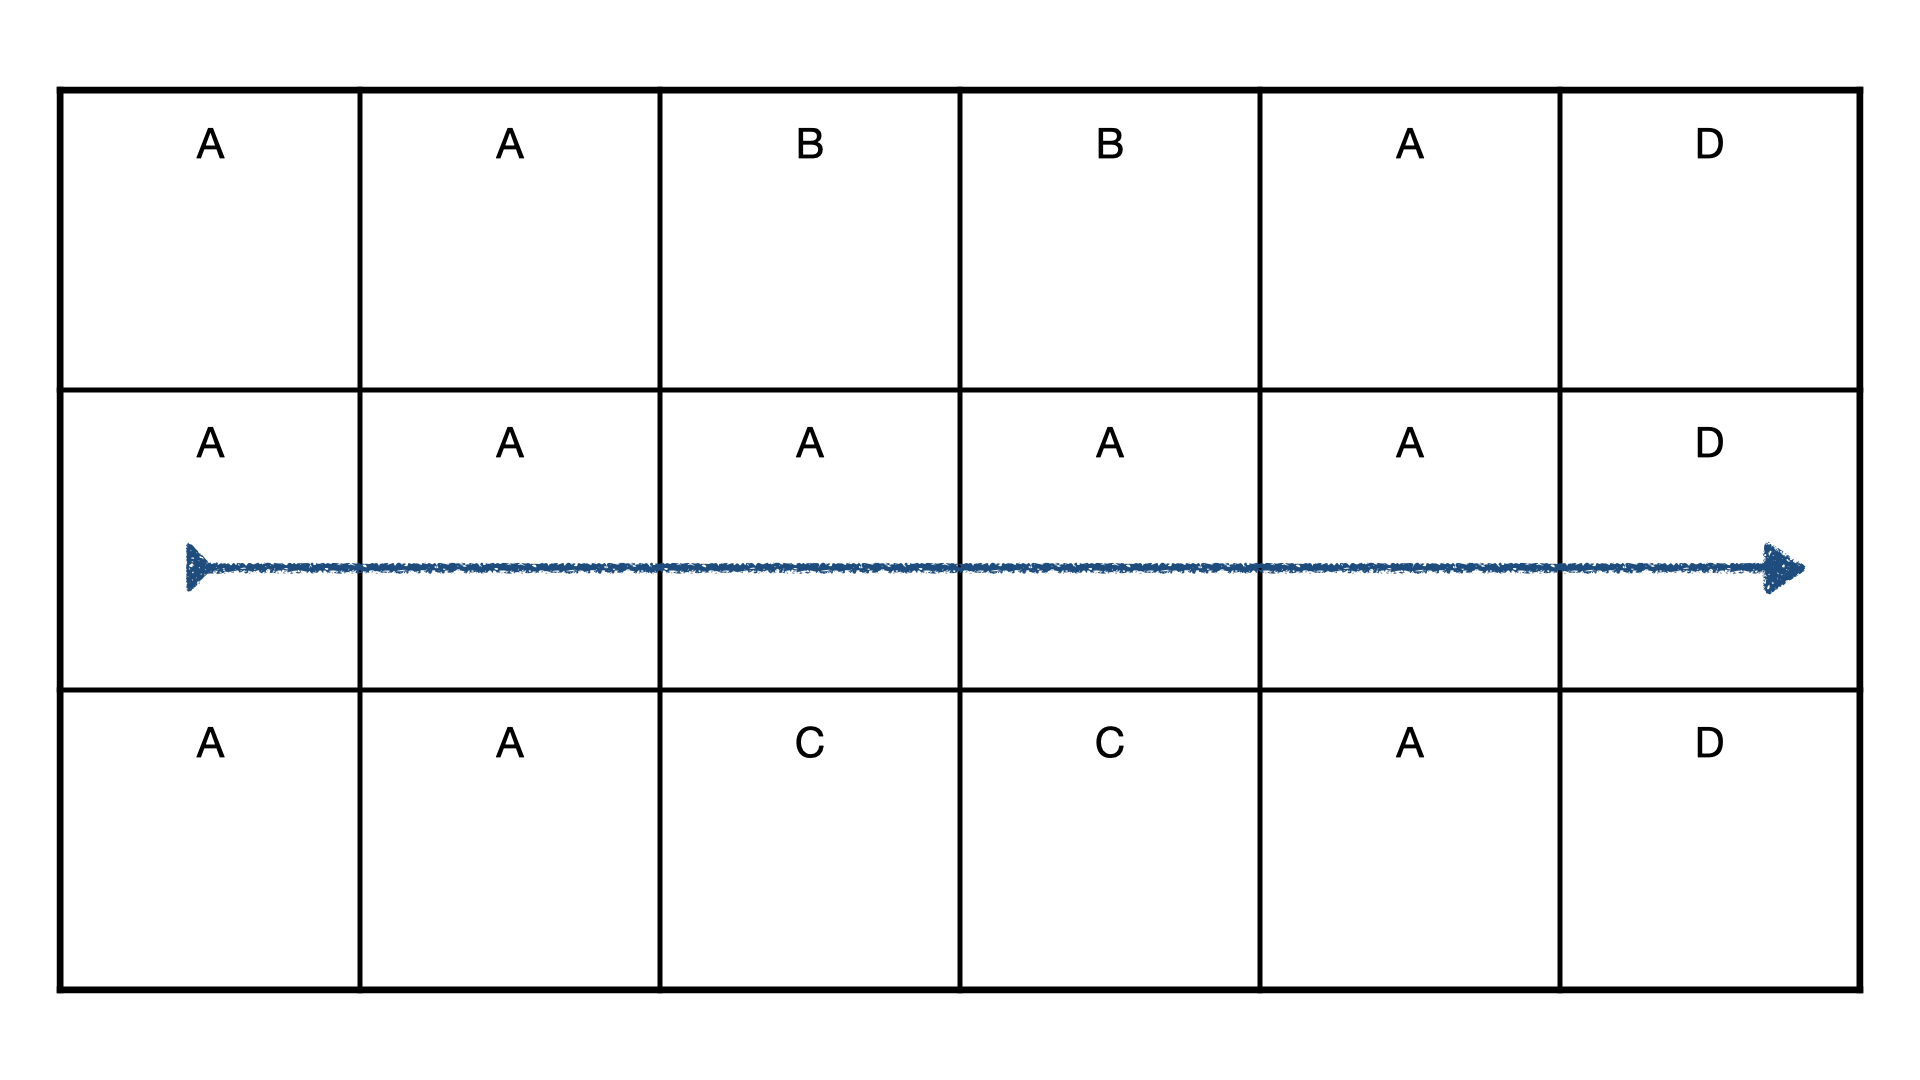
\includegraphics[scale=0.1]{draw/Thesis_plots/Thesis_plots.004}
\captionsetup{width=.8\linewidth}
\caption{A straight path. This path is forced to go straight right because of the distribution $A$ that permits only this movement.}
\label{fig:simplistic_example_4}
\end{minipage}
\begin{minipage}[c]{0.5\linewidth}
\centering
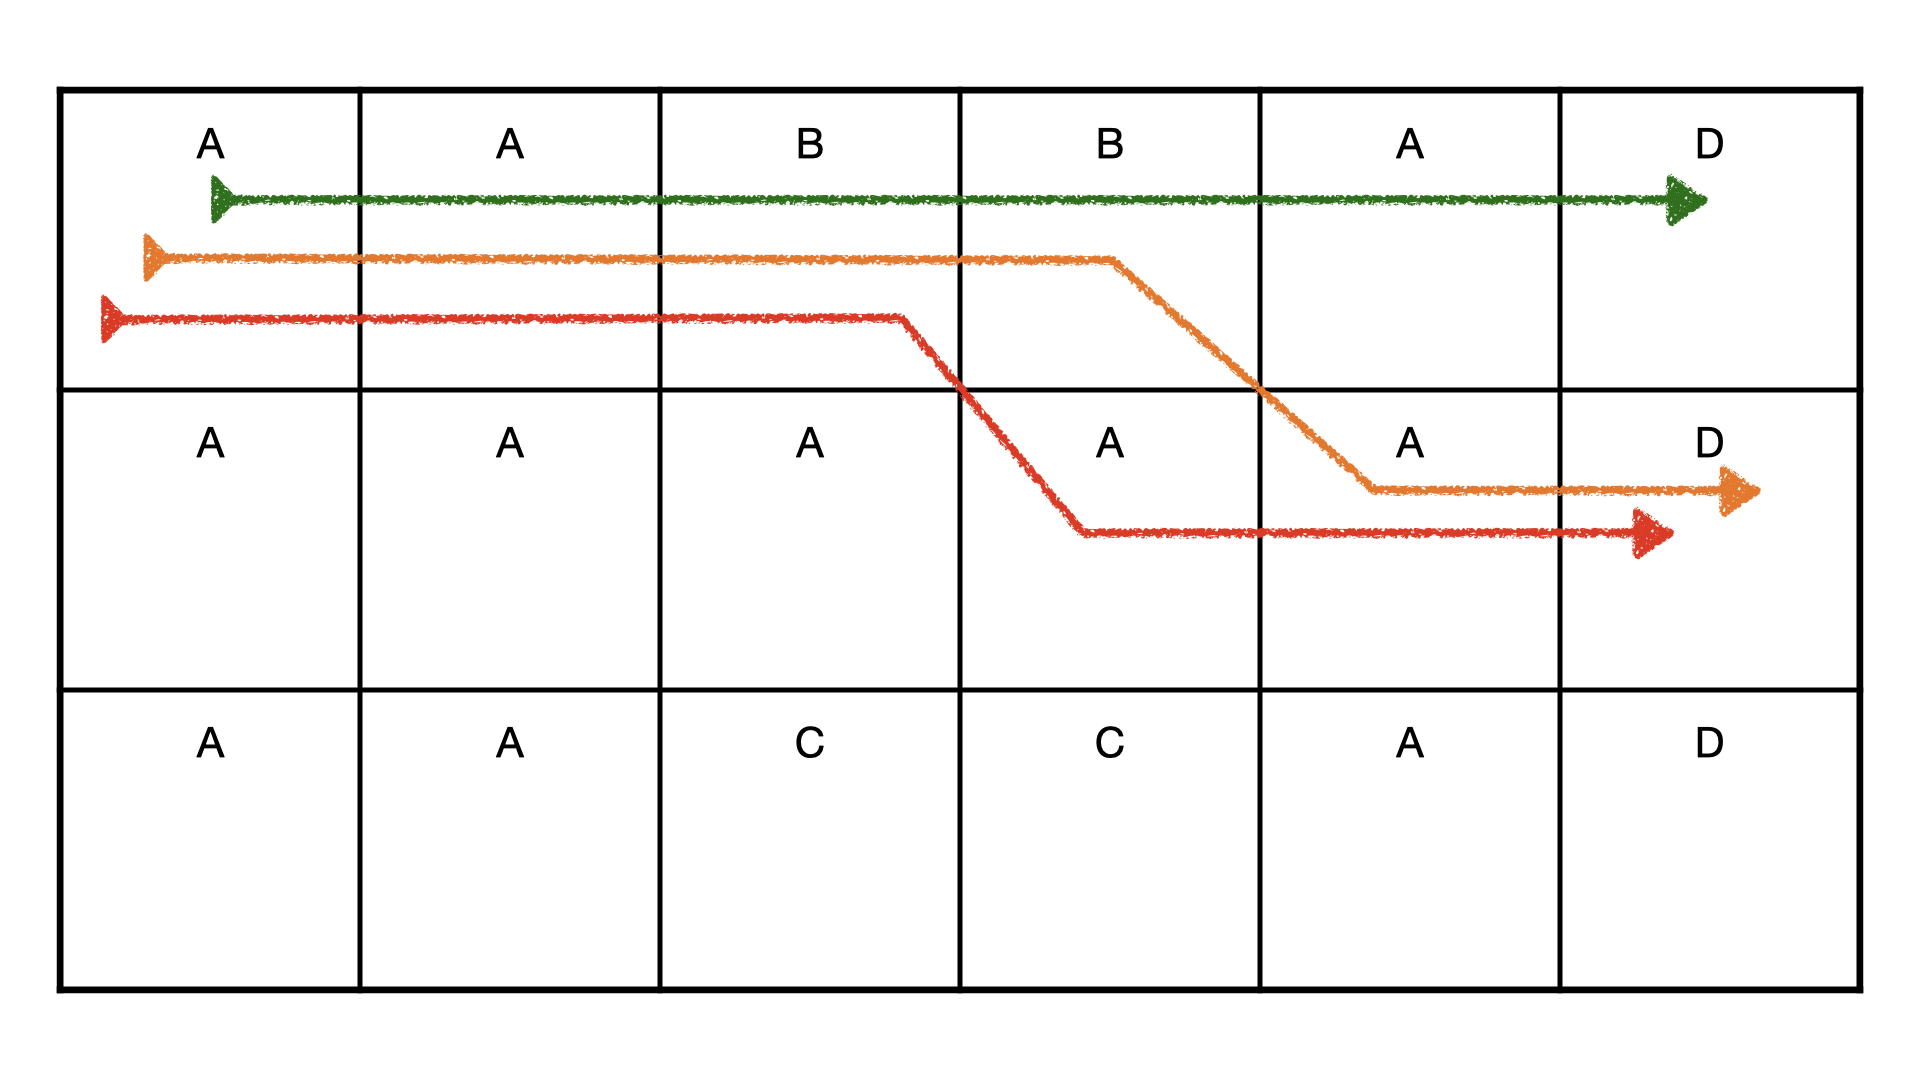
\includegraphics[scale=0.1]{draw/Thesis_plots/Thesis_plots.005}
\captionsetup{width=.8\linewidth}
\caption{The three possible paths when starting from the upper-left cell. This situation is specular to when starting from the bottom-left cell.}
\label{fig:simplistic_example_5}
\end{minipage}
\end{figure}

\paragraph{Real-life situation}
The previous example is a simplification of a real study case.
It is easy enough to calculate by hand the possibles paths.
The dataset showed before in (Figure \ref{fig:5pids_trjlines}) has a grid space dimensions of $200 \times 100$ cells.
In that real scenario, the field $\Omega_g$ is larger than the simplified example of the previous paragraph.
The grid dimensions depend always on two factors: the physical space dimensions (in meters) and the choice of the grid size.
The (Figure \ref{fig:5pids_D2Q9}) express the values of each direction in correlation to the map position.
That figure is strictly liked to the matrices shown in (Equation \ref{equation:simplistic_example_transitions}), but this is referred to the real case.
Even this scenario is simplified because it takes into account only five trajectories.
For comparison, let's consider the entire dataset, (Figure \ref{fig:TensorA_D2Q9}) shows how complex may become the representation when these transitions are calculated for a greater multitude of real pedestrian trajectories.
\\Taking into account a Real-life situation as an example, with 3210 trajectories.
The data representation would be as in (Figure \ref{fig:3210_L} - \ref{fig:3210_3x3}).

\begin{figure}[ht]
\begin{minipage}[c]{0.5\linewidth}
\centering
\includegraphics[ width=1\textwidth]{fig/3210pids/figure_trainf10_RealData_lines_postTrans_NumP_3210_}
\captionsetup{width=.8\linewidth}
\caption{Plot L: 3210 pedestrian's trajectories.}
\label{fig:3210_L}
\end{minipage}
\begin{minipage}[c]{0.5\linewidth}
\centering
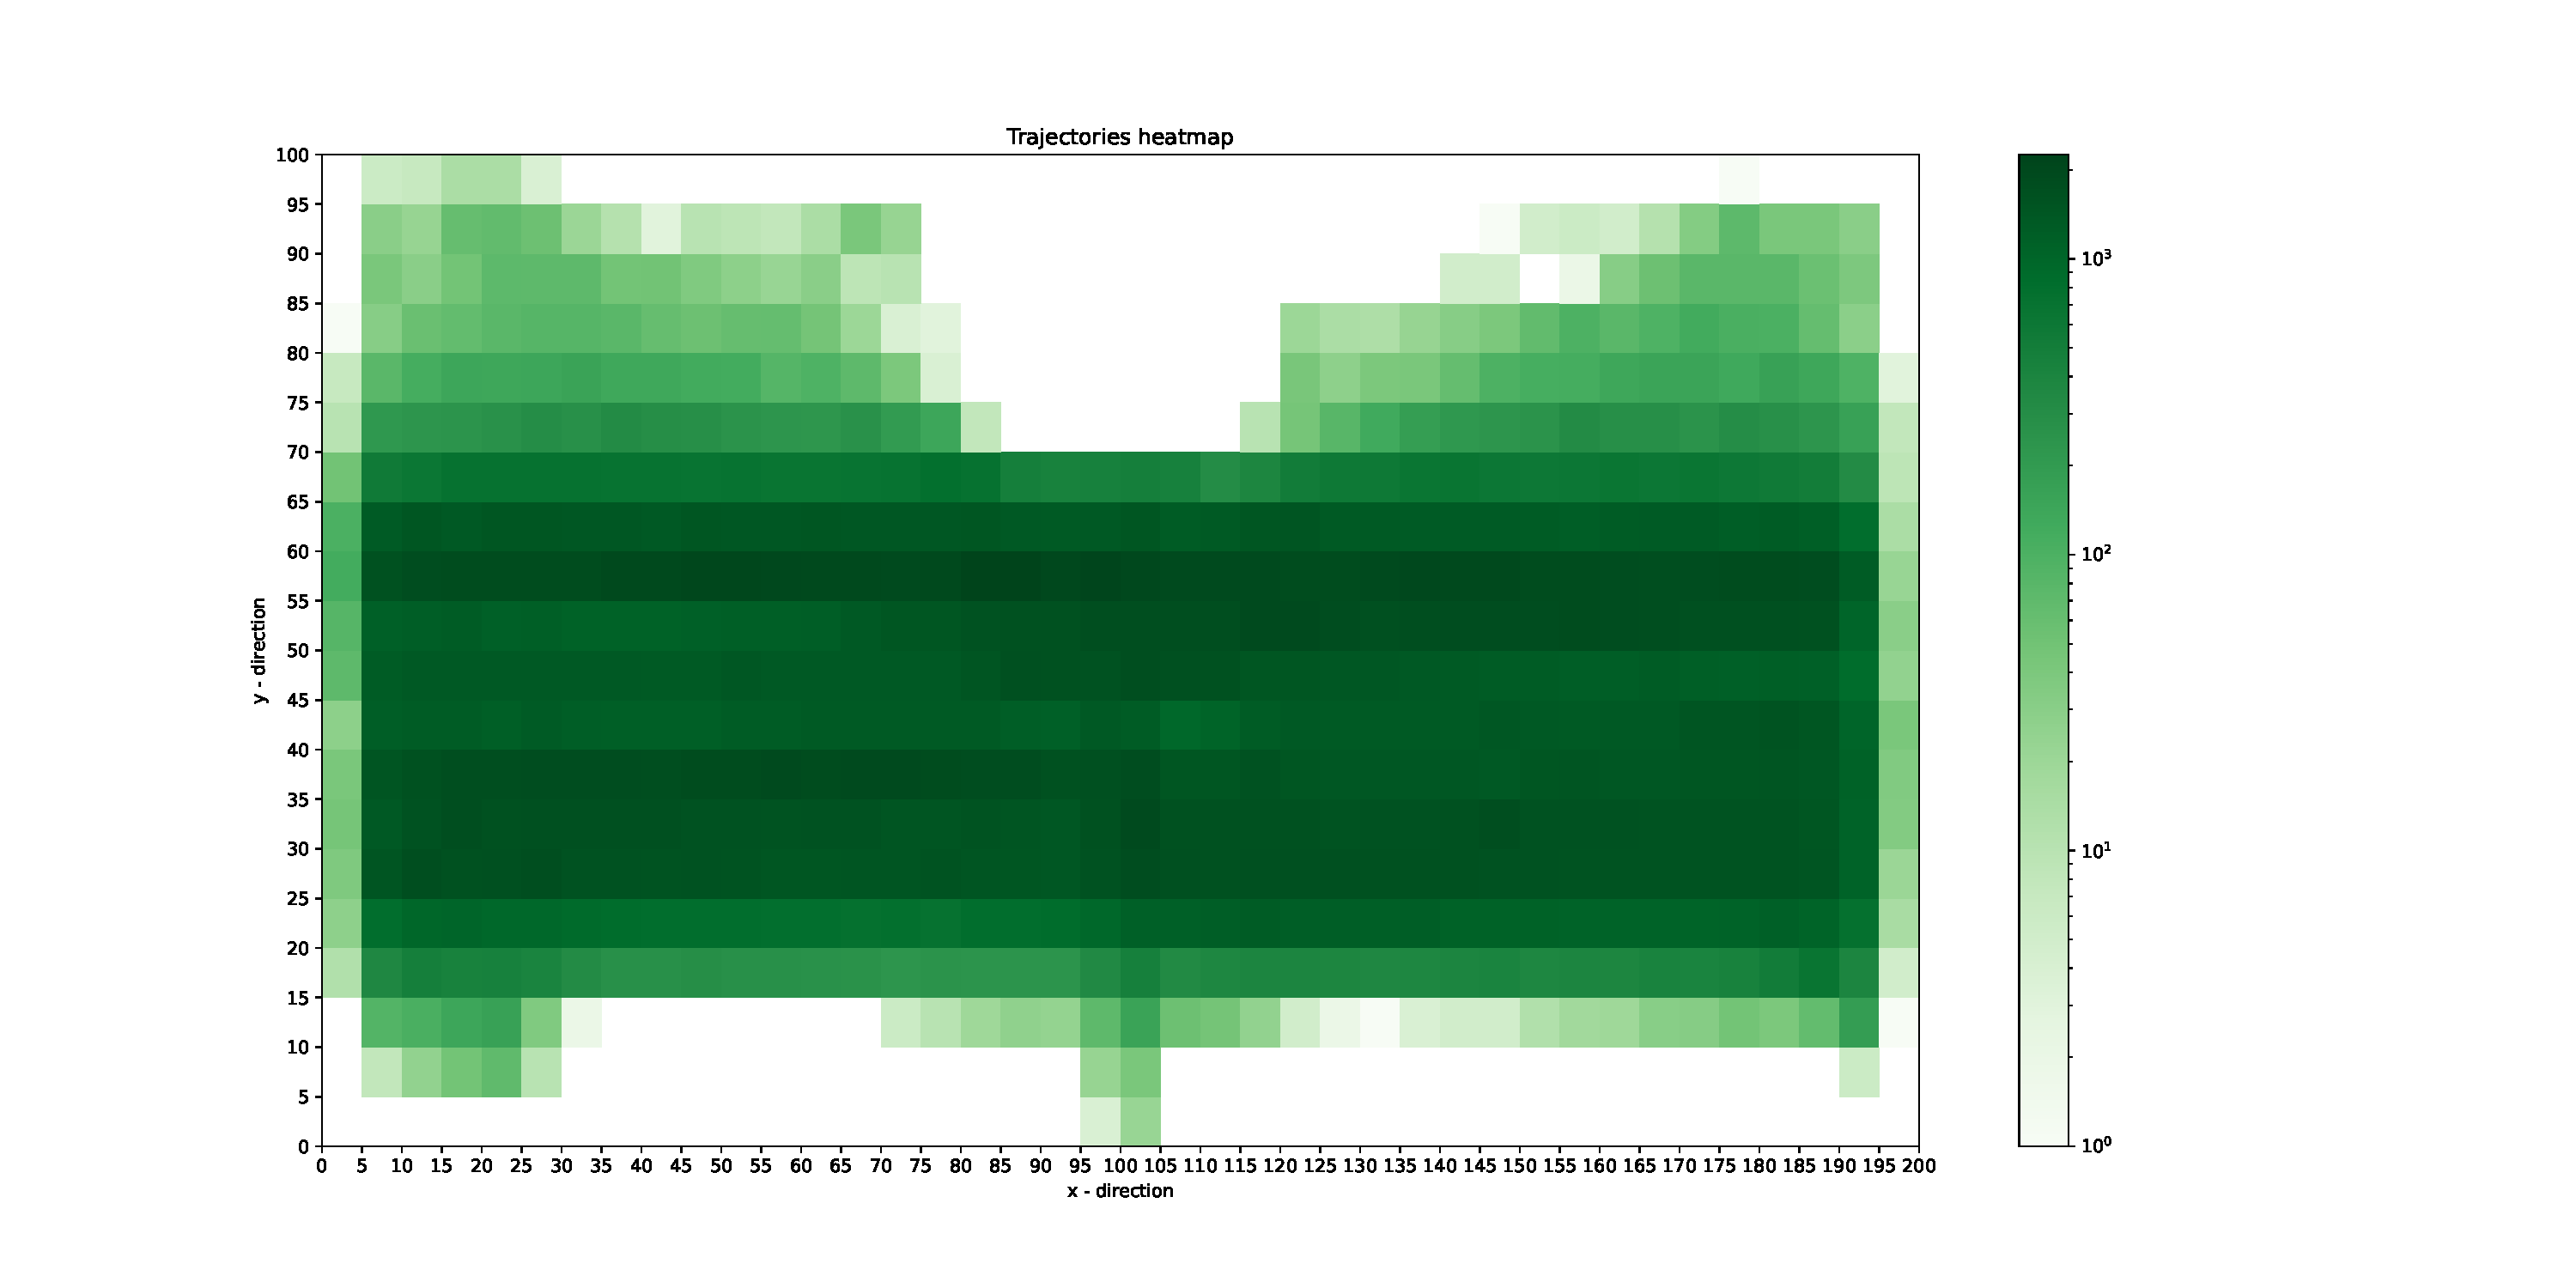
\includegraphics[ width=1\textwidth]{fig/3210pids/figure_trainf10_RealData_heatmap_postTrans_NumP_3210_}
\captionsetup{width=.8\linewidth}
\caption{Plot H: 3210 pedestrian's trajectories.}
\label{fig:3210_H}
\end{minipage}
\vspace*{5mm}
\begin{minipage}[c]{0.35\linewidth}
\centering
\includegraphics[ width=0.95\textwidth]{fig/3210pids/figure_trainf10_RealData_velocity_heatmap_postTrans_NumP_3210_}
\captionsetup{width=.8\linewidth}
\caption{Plot V: 3210 pedestrian's trajectories.}
\label{fig:3210_V}
\end{minipage}
\begin{minipage}[c]{0.65\linewidth}
\centering
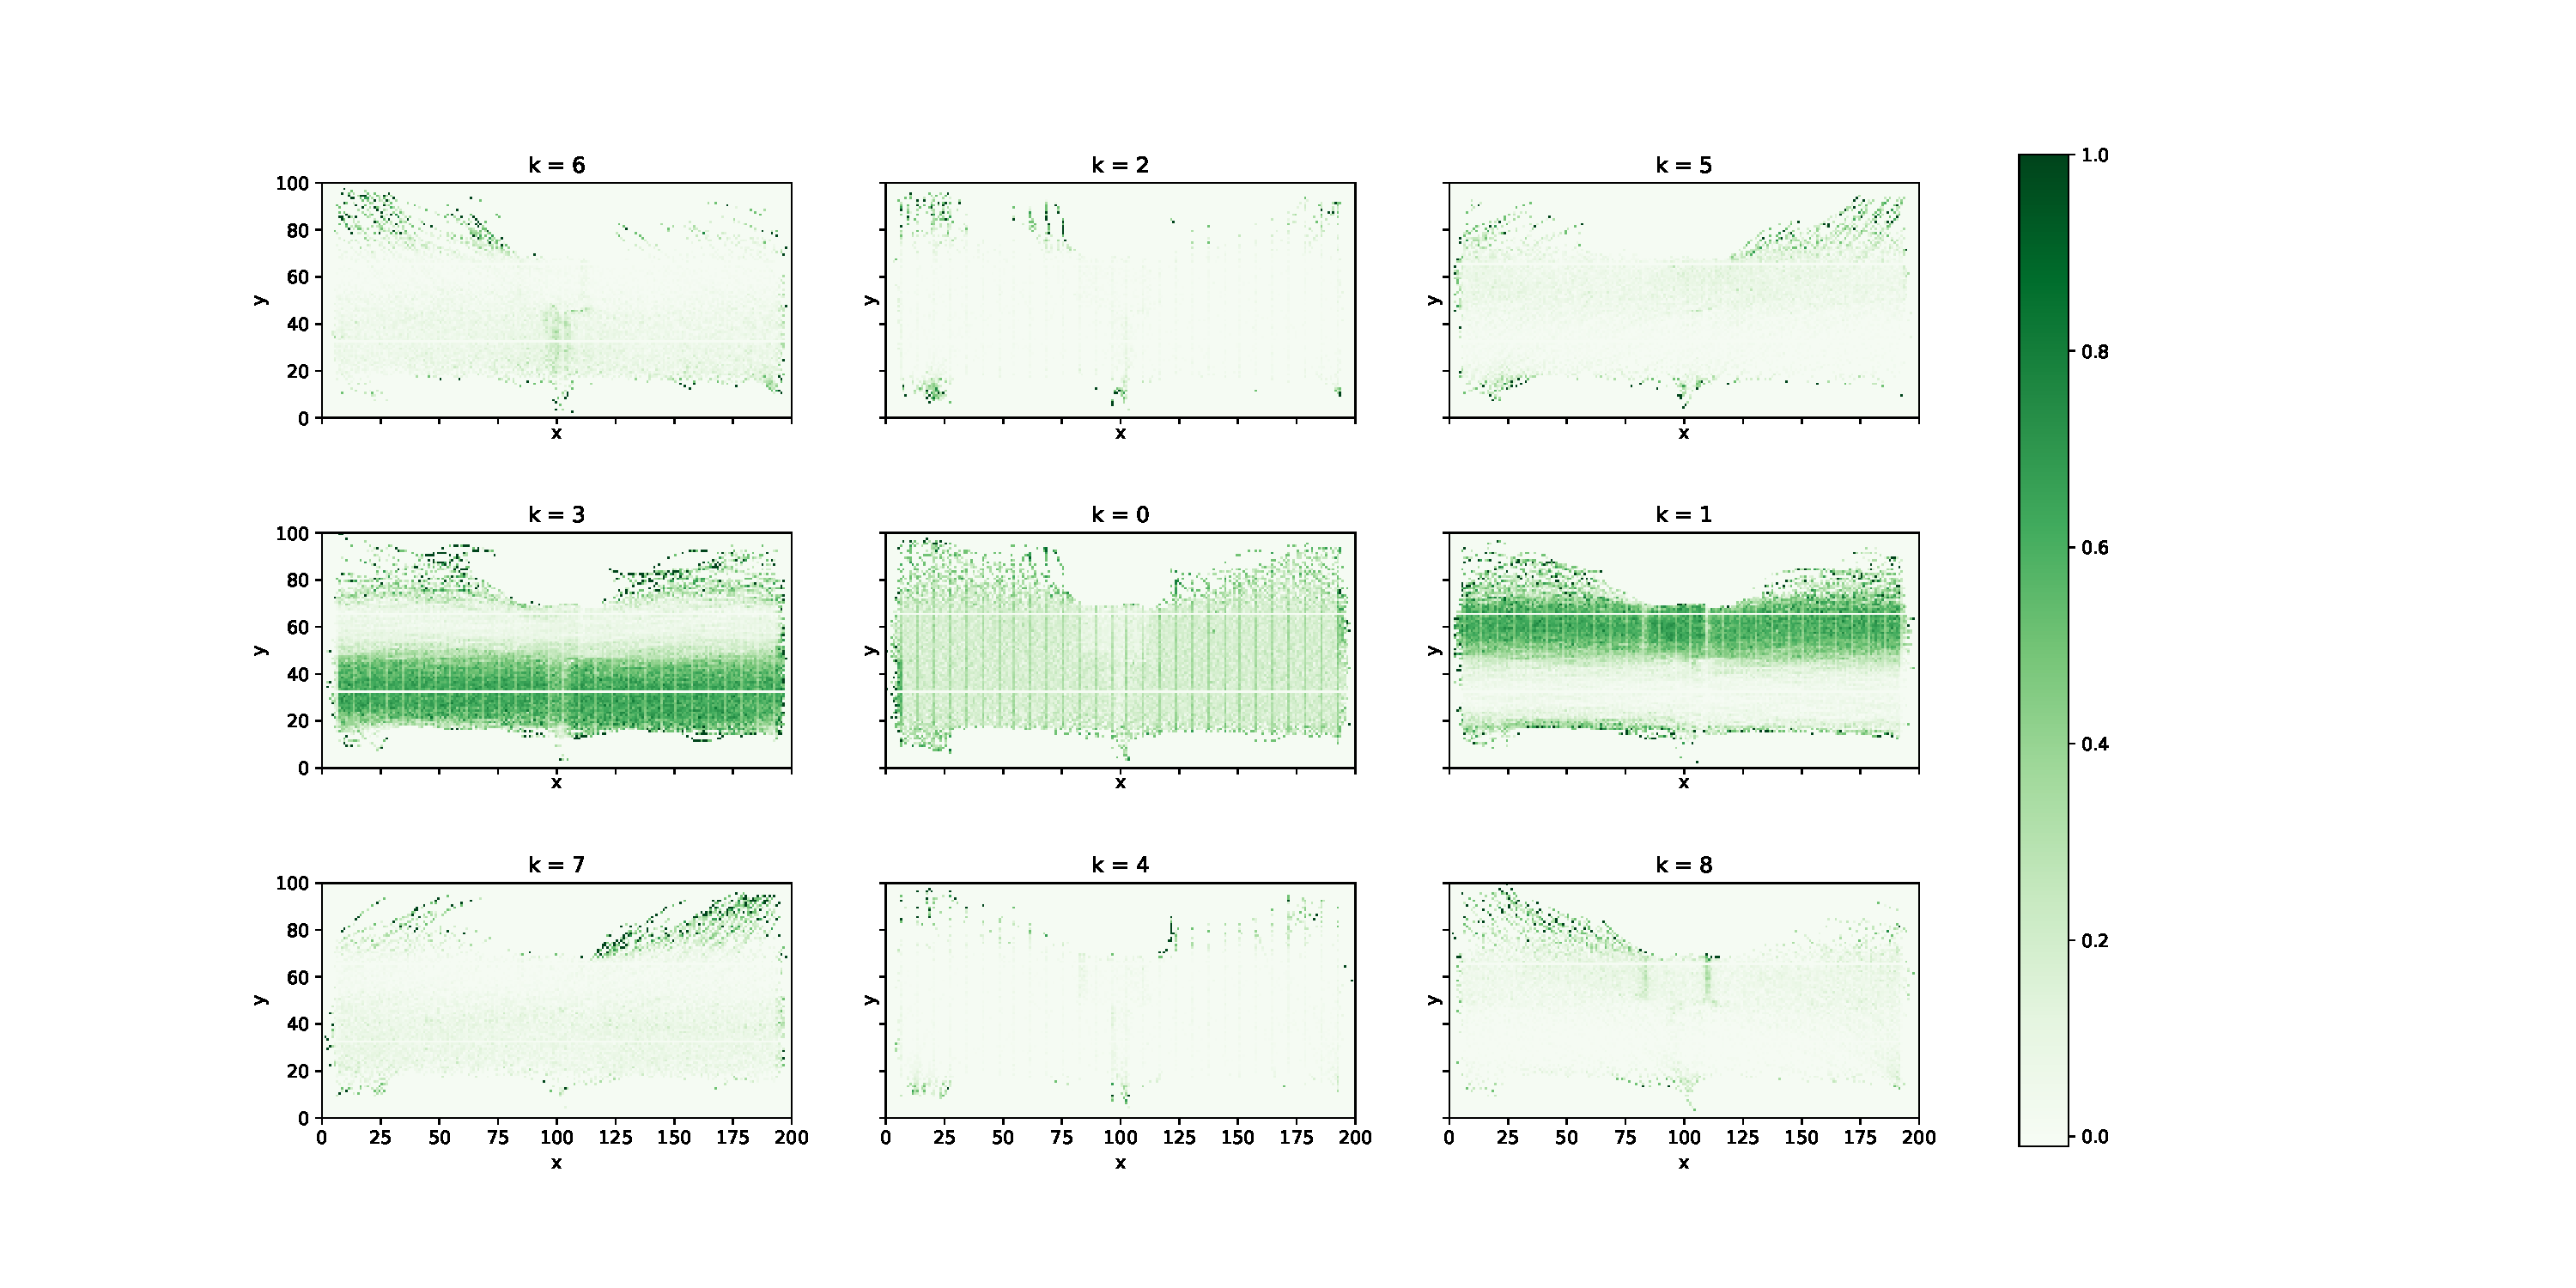
\includegraphics[ width=1\textwidth]{fig/3210pids/figure_trainf10__D2Q9nA_all_3x3}
\captionsetup{width=.8\linewidth}
\caption{Plot of D2Q9's $k$-index: 3210 pedestrian's trajectories.}
\label{fig:3210_3x3}
\end{minipage}
\end{figure}




\end{document}
